\documentclass{beamer}
\usepackage[utf8]{inputenc}
\usepackage{booktabs}
\usepackage{slovak}
\usetheme{Warsaw}
\title{Biologicky motivované \\výpočtové modely}
\author{Michal Kováč}
\institute{FMFI UK}
\date{24.6.2013}
\begin{document}

\begin{frame}[t]
\titlepage
\end{frame}

\section*{Outline}
\begin{frame}
\tableofcontents
\end{frame}

\section{Prehľad problematiky} % (fold)
\label{sec:prehlad_problematiky}

\subsection{Prehľad modelov} % (fold)
\label{sub:prehlad_modelov}

\begin{frame}[t]\frametitle{Biologicky motivované\\výpočtové modely}
Modely vznikajú s dvoma účelmi:
\begin{itemize}
  \item simulácia biologických javov
  \item zdokonalenie informatických riešení
\end{itemize}
\end{frame}

\begin{frame}[t]\frametitle{Biologicky motivované\\výpočtové modely}
\begin{itemize}
  \item Neurónové siete (od 1943)
  \item Celulárne automaty (od 1948)
  \item Evolučné algoritmy (od 1954)
  \item L systémy (od 1968)
  \item P systémy (od 1998) \cite{Paun98}
  \item \dots
\end{itemize}
\end{frame}

% subsection prehlad_modelov (end)

\subsection{P systémy} % (fold)
\label{sub:p_systemy}

\begin{frame}[t]\frametitle{Membránová štruktúra}
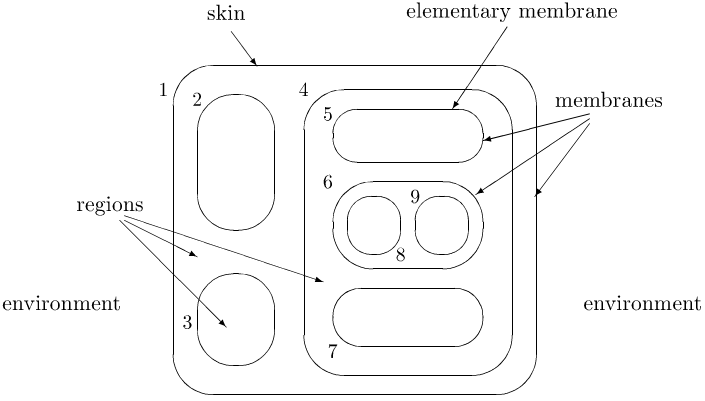
\includegraphics[width=0.7\textwidth]{membrane_structure.png}
\hfill
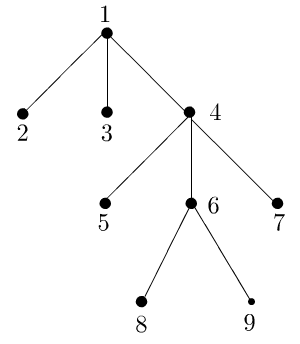
\includegraphics[width=0.3\textwidth]{membrane_tree.png}
\end{frame}

\begin{frame}[t]\frametitle{Obsah membrány}
\begin{itemize}
  \item multimnožina objektov
  \begin{itemize}
    \item $a\ |\ b\ |\ b$
  \end{itemize}
  \item prepisovacie pravidlá
  \begin{itemize}
    \item $a\ |\ b\ |\ b\rightarrow a\ |\ a\downarrow\ |\ a\uparrow\ |\ b\downarrow_6$
    \item $b \rightarrow a\ |\ \delta$
  \end{itemize}
\end{itemize}
\end{frame}

\begin{frame}[t]\frametitle{P systém}

P systém definujeme ako $\Pi = (V, \mu, w_1, w_2,\dots , w_m, R_1, R_2, \dots , R_m)$, kde:
\begin{itemize}
  \item $V$ je abeceda objektov
  \item $\mu$ je membránová štruktúra
  \item $w_1, w_2, \dots w_m$ sú počiatočné multimnožiny v membránach $1\dots m$, $w_i\subseteq \mathbb{N}^V$
  \item $R_1, R_2, \dots , R_m$ sú množiny prepisovacích pravidiel v membránach $1\dots m$, pričom $$R_i\subseteq(\mathbb{N}^V\setminus 0^V)\times\mathbb{N}^{V\times(\{here,in,out\}\cup\{in_1,\dots in_m\})}$$.
\end{itemize}

\end{frame}

\begin{frame}[t]\frametitle{Konfigurácia a krok výpočtu}
\begin{itemize}
  \item konfigurácia = membránová štruktúra + obsahy membrán
  \item krok výpočtu: maximálny paralelizmus
\end{itemize}

\begin{align*}
  a\ |\ b\ |\ b&\rightarrow c\\
  b &\rightarrow c\ |\ c\\
  a\ |\ a\ |\ b\ |\ b\\\midrule
  \onslide<2->{a\ |\ c\\\midrule
  a\ |\ a\ |\ c\ |\ c}
\end{align*}
\end{frame}

\begin{frame}[t]\frametitle{Jazyk}
\begin{itemize}
  \item Parikhovo zobrazenie
  \item alternatíva: worm objects \cite{Mate02}
  \begin{itemize}
    \item namiesto multimnožín objektov sú v membránach multimnožiny stringov
    \item inšpirované DNA
  \end{itemize}

  \item generatívny mód
  \item akceptačný mód
\end{itemize}
\end{frame}

% subsection p_systemy (end)

\subsection{Varianty} % (fold)
\label{sub:varianty}

\begin{frame}[t]\frametitle{Varianty pravidiel}
\begin{itemize}
  \item kontextové (PsRE)
  \item kooperatívne (PsRE)
  \item katalytické
  \begin{itemize}
    \item s 2 katalyzátormi (PsRE) \cite{Freund2005TwoCatalysts}
    \item s 1 katalyzátorom (otvorený problem)
    \item s 1 katalyzátorom a inhibítormi (PsRE) \cite{Ionescu:jucs_10_5:on_p_systems_with}
  \end{itemize}
  \item bezkontextové (PsCF) \cite{Sburlan05dragos}
  \item bezkontextové s inhibítormi (PsET0L) \cite{Ionescu:jucs_10_5:on_p_systems_with}
\end{itemize}
\end{frame}

\begin{frame}[t]\frametitle{Varianty kroku výpočtu}
\begin{itemize}
  \item maximálny paralelizmus (PsRE)
  \item maximálny paralelizmus bez priorít (PsRE) \cite{Sosik:2002:WithoutPriorities}
  \item sekvenčný (vieme simulovať pomocou VASS, \cite{Dang:2005:Sequential})
  \item sekvenčný s prioritami (TODO)
  \item asynchrónny (TODO)
  \item minimálny paralelizmus (PsRE) \cite{Ciobanu:2007:MinimalParallelism}
  \item n-paralelizmus, max-n-paralelizmus, \dots
\end{itemize}
\end{frame}

% subsection varianty (end)

% section prehlad_problematiky (end)

\section{Plány na dizertačnú prácu} % (fold)
\label{sec:plany_na_dizertacnu_pracu}

\subsection{Aktuálne riešené problémy} % (fold)
\label{sub:aktualne_riesene_problemy}

\begin{frame}[t]\frametitle{Sekvenčné P systémy}
\begin{itemize}
  \item nie sú univerzálne
  \item na univerzalitu treba:
  \begin{itemize}
    \item povoliť neobmedzené vytváranie membrán \cite{Dang:2005:Sequential}
    \item inhibítory
      \begin{itemize}
        \item publikuje sa
        \item Inhibiting the parallelism in P systems
        \item 2nd International Workshop on Hybrid Systems and Biology
      \end{itemize}
    \item iné rozšírenia (vacuum, ...)
    \item inšpirácie z výsledkov iných formalizmov
  \end{itemize}
\end{itemize}
\end{frame}

% subsection aktualne_riesene_problemy (end)

\subsection{Ďalšie plány} % (fold)
\label{sub:dalsie_plany}

\begin{frame}[t]\frametitle{Ďalšie plány}
\begin{itemize}
  \item Preskúmať možnosti kombinovania ďalších variantov P systémov z hľadiska výpočtovej sily
  \begin{itemize}
    \item priestorové P systémy
    \item rozpadajúce sa objekty
    \item energie
  \end{itemize}
  \item Porovnať s inými formalizmami, napríklad Petriho siete / reaction systems / CLS / ...
  \item Nájsť nové varianty
\end{itemize}
\end{frame}


\begin{frame}[t]\frametitle{Inšpirácie z výsledkov iných formalizmov}
\begin{itemize}
  \item Petriho siete
  \begin{itemize}
    \item nie sú univerzálne
    \item s inhibítormi áno
    \item ake iné varianty Petriho sietí ešte nikto nevyskúšal aplikovať v P systémoch?
  \end{itemize}
  \item CLS (Calculi of Looping Sequences)
  \begin{itemize}
    \item sekvenčný model, vie simulovať P systémy \cite{Barbuti07CLS}
  \end{itemize}
  \item Reakčné (alebo reaktívne?) systémy
\end{itemize}
\end{frame}

\begin{frame}[t]\frametitle{Nové varianty}
Besozzi \cite{Besozzi:PhD:2004}: Dobrý variant by mal byť:
\begin{itemize}
  \item realistický
  \item univerzálny
  \item iredundantný
\end{itemize}
\end{frame}

% subsection dalsie_plany (end)

% section plany_na_dizertacnu_pracu (end)

\begin{frame}[allowframebreaks]{Literatúra}
\bibliographystyle{apalike}
\bibliography{presentation.bib}
\end{frame}

\begin{frame}[plain]
\begin{center}
  Ďakujem za pozornosť
\end{center}
\end{frame}

\end{document}